\section{Introduction}
\label{sec:introduction}


\par The objective of this laboratory assignment was to create a circuit that would transform an input AC voltage of amplitude 230V and frequency of 50 Hz to an output DC voltage of amplitude 12V and frequency 50Hz.To do this an Envelope detector, a Voltage Regulator and a Transformer were used. This last component was not actually modeled in the simulation and theorethical analysis. It was considerared that the transformer would be represented whith an alternated voltage source that would connect to the envelope detector and would reduce the amplitude of the first source in a ratio of n:1.This ratio will be decided during the simulation and theorethical analysis.\par
To determine whether or not the circuit was good when compared to others a merit classification sistem was created. This merit sistem took into account the cost of the components used and the ripple and average amplitude of the output voltage.The merit of the circuit will determined according to the following equation: 
\begin {equation}
	MERIT = \dfrac{1}{cost*(ripple_reg + abs(average_reg - 12) + 1e-6)}	
	\label{eq:i1}
\end{equation}

and the cost of the componets are the following: cost of resistors = 1 monetary unit (MU) per kOhm, cost of capacitors = 1 MU/uF
and cost of diodes = 0.1 MU per diode. The voltage source that represents the transformer was not taken into account in the cost. 
 
The circuit that was implemented can be seen in \textbf{Figure~\ref{fig:circuit_t3}}.\par
\begin{figure}[h] \centering
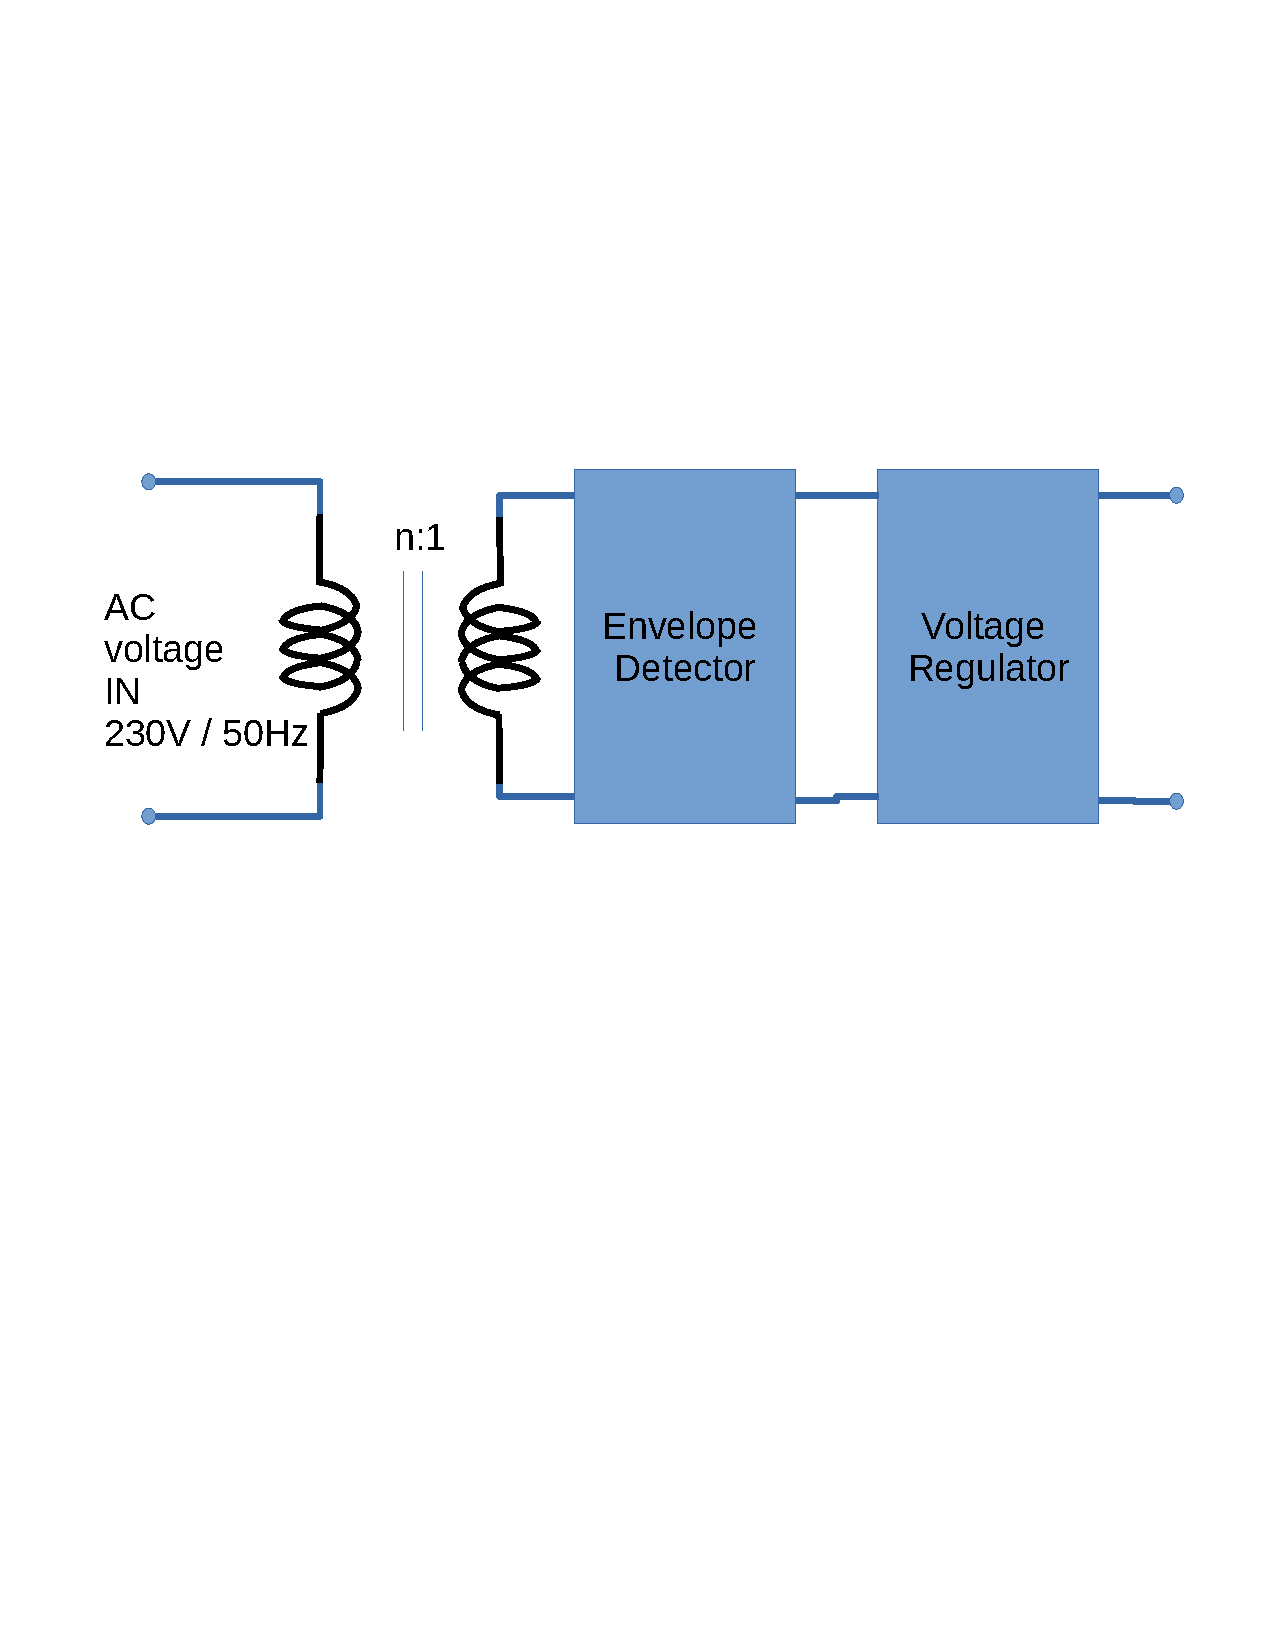
\includegraphics[width=0.4\linewidth]{circuit_t3.pdf}
\caption{Circuit in study}
\label{fig:circuit_t3}
\end{figure}


In Section~\ref{sec:analysis}, a theoretical analysis of the circuit is
presented. Here the circuit is analised using suitbale theorethicals models for the diodes in order to predict the output of the Envelope Detector
and Voltage Regulator circuits. The output DC level and the
voltage ripple are calculated and the plots for the voltages at the output of the Envelope Detector and Voltage Regulator circuits are presented, as well as the plot for the diference between the output of the regulator with 12. 
In Section~\ref{sec:simulation}, the circuit is analysed by
simulation using the program Ngspice.In Ngspice de default model for the diode was used. The AC/DC converter was simulated for 10 periods and the voltage average and ripple were mesured using built in functions of the program.The same plots produced in the theoretical analysis were made in this section by simultaion.The conclusions of this study are outlined in
Section~\ref{sec:conclusion}, where the theoretical results obtained in
Section~\ref{sec:analysis} are compared to the simulation results obtained in
Section~\ref{sec:simulation}.





\pagebreak

